%
% Annual Cognitive Science Conference
% Sample LaTeX Paper -- Proceedings Format
%
% Original : Ashwin Ram (ashwin@cc.gatech.edu)       04/01/1994
% Modified : Johanna Moore (jmoore@cs.pitt.edu)      03/17/1995
% Modified : David Noelle (noelle@ucsd.edu)          03/15/1996
% Modified : Pat Langley (langley@cs.stanford.edu)   01/26/1997
% Latex2e corrections by Ramin Charles Nakisa        01/28/1997
% Modified : Tina Eliassi-Rad (eliassi@cs.wisc.edu)  01/31/1998
% Modified : Trisha Yannuzzi (trisha@ircs.upenn.edu) 12/28/1999 (in process)
% Modified : Mary Ellen Foster (M.E.Foster@ed.ac.uk) 12/11/2000
% Modified : Ken Forbus                              01/23/2004
% Modified : Eli M. Silk (esilk@pitt.edu)            05/24/2005
% Modified : Niels Taatgen (taatgen@cmu.edu)         10/24/2006
% Modified : David Noelle (dnoelle@ucmerced.edu)     11/19/2014

%% Change ''letterpaper'' in the following line to ''a4paper'' if you must.

\documentclass[10pt,letterpaper]{article}

\usepackage{cogsci}
\usepackage{pslatex}
\usepackage{apacite}
\usepackage{amsmath,amssymb}
\usepackage{graphicx}
\usepackage{subcaption}
\usepackage{caption}
\captionsetup{font=footnotesize}
\usepackage{color}
\usepackage{url}
\usepackage{todonotes}
\usepackage{mathtools}
\usepackage{stmaryrd}
\usepackage{booktabs}
\usepackage{array}
\usepackage{nicefrac}

\graphicspath{{./figures/}}

%\newcommand{\url}[1]{$#1$}

\definecolor{Red}{RGB}{178,34,34}
\definecolor{Green}{RGB}{10,200,100}
\definecolor{Blue}{RGB}{10,50,150}

\hyphenpenalty=1000

\newcommand{\jefan}[1]{\textcolor{Blue}{jefan: #1}}
\newcommand{\rdh}[1]{\textcolor{Red}{rdh: #1}}
\newcommand{\denote}[1]{\mbox{ $[\![ #1 ]\!]$}}
\newcommand{\subsubsubsection}[1]{{\em #1}}
\newcommand{\eref}[1]{(\ref{#1})}
\newcommand{\tableref}[1]{Table \ref{#1}}
\newcommand{\figref}[1]{Fig.~\ref{#1}}
\newcommand{\appref}[1]{Appendix \ref{#1}}
\newcommand{\sectionref}[1]{Section \ref{#1}}

\title{Graphical convention formation during visual communication}

% \author{\begin{tabular}[htbp]{c@{\extracolsep{1em}}c@{\extracolsep{1em}}c@{\extracolsep{1em}}c} \\
% {\large \bf Robert X. D. Hawkins*} & {\large \bf Megumi Sano*} & {\large \bf Noah D. Goodman} & {\large \bf Judith E. Fan}\\
% Department of Psychology & Department of Psychology & Department of Psychology & Department of Psychology \\
% Stanford University & Stanford University & Stanford University & UC San Diego \\
% \texttt{rxdh@stanford.edu} & \texttt{megsano@stanford.edu} & \texttt{ngoodman@stanford.edu} & \texttt{jefan@ucsd.edu} \\
% \end{tabular}
% }

\author{\large \bf Anonymous Authors}

\begin{document}
\maketitle

\begin{abstract}
Drawing is a versatile technique for visual communication, ranging from photorealistic renderings to schematic diagrams consisting entirely of symbols.
How does a medium spanning such a broad range of appearances reliably convey meaning?
A natural possibility is that drawings derive meaning from both their visual properties as well as shared knowledge between people who use them to communicate.
Here we evaluate this possibility in a drawing-based reference game in which two participants repeatedly communicated about visual objects.
% by investigating how the accumulation of shared knowledge influences the drawings they produce and how well they communicate
Across a series of controlled experiments, we found that pairs discover increasingly sparse yet effective ways of depicting them.
These gains were specific to those objects that were repeatedly referenced, and went beyond what could be explained by task practice or the visual properties of the drawings alone.
We employed modern techniques from computer vision to characterize how the high-level visual features of drawings changed, finding that drawings of the same object became more consistent within a pair and divergent across different pairs.
Taken together, these findings suggest that visual communication promotes the emergence of depictions whose meanings are increasingly determined by shared knowledge rather than their visual properties alone.

\textbf{Keywords:}
drawing understanding; alignment; drawing; iconicity; visual abstraction

% On each trial, both players were shown an array of objects; the sketcher’s goal was to draw one of these, the target, so that the viewer could guess the target as quickly as possible.
% The game included two sets of objects: objects in one set were drawn repeatedly, while those in a control set were drawn once at the beginning and again at the end of the game.
% While we observe gains in communication efficiency for all objects, they were greater for the repeated objects, suggesting both task-level and object-level benefits of repeated communication.
% Moreover, different pairs discovered different solutions for efficient communication, suggesting the existence of multiple equilibria in the space of viable graphical conventions.

\end{abstract}


\section{Introduction}

From ancient etchings on cave walls to modern digital displays, visual communication lies at the heart of key human innovations (e.g., cartography, data visualization) and forms a durable foundation for the cultural transmission of knowledge and higher-level reasoning.
Perhaps the most basic and versatile technique supporting visual communication is drawing, the earliest examples of which date to at least 40,000-60,000 years ago \cite{hoffmann2018u}. 
What began as simple mark making since been adapted to a wide array of applications, ranging between photorealistic rendering from observation to schematic diagrams consisting entirely of symbols.

Even drawings of the same object can be highly variable.
How does a communication medium spanning such a broad range of appearances reliably convey meaning?
On the one hand, prior work has found that semantic information in a figurative drawing, i.e., the object it represents, can be derived purely from its visual properties \cite{FanCommon2018}.
On the other hand, other work has emphasized the role of socially-mediated information and context for making appropriate inferences about what even a figurative drawing represents \cite{goodman1976languages}.

\begin{figure}
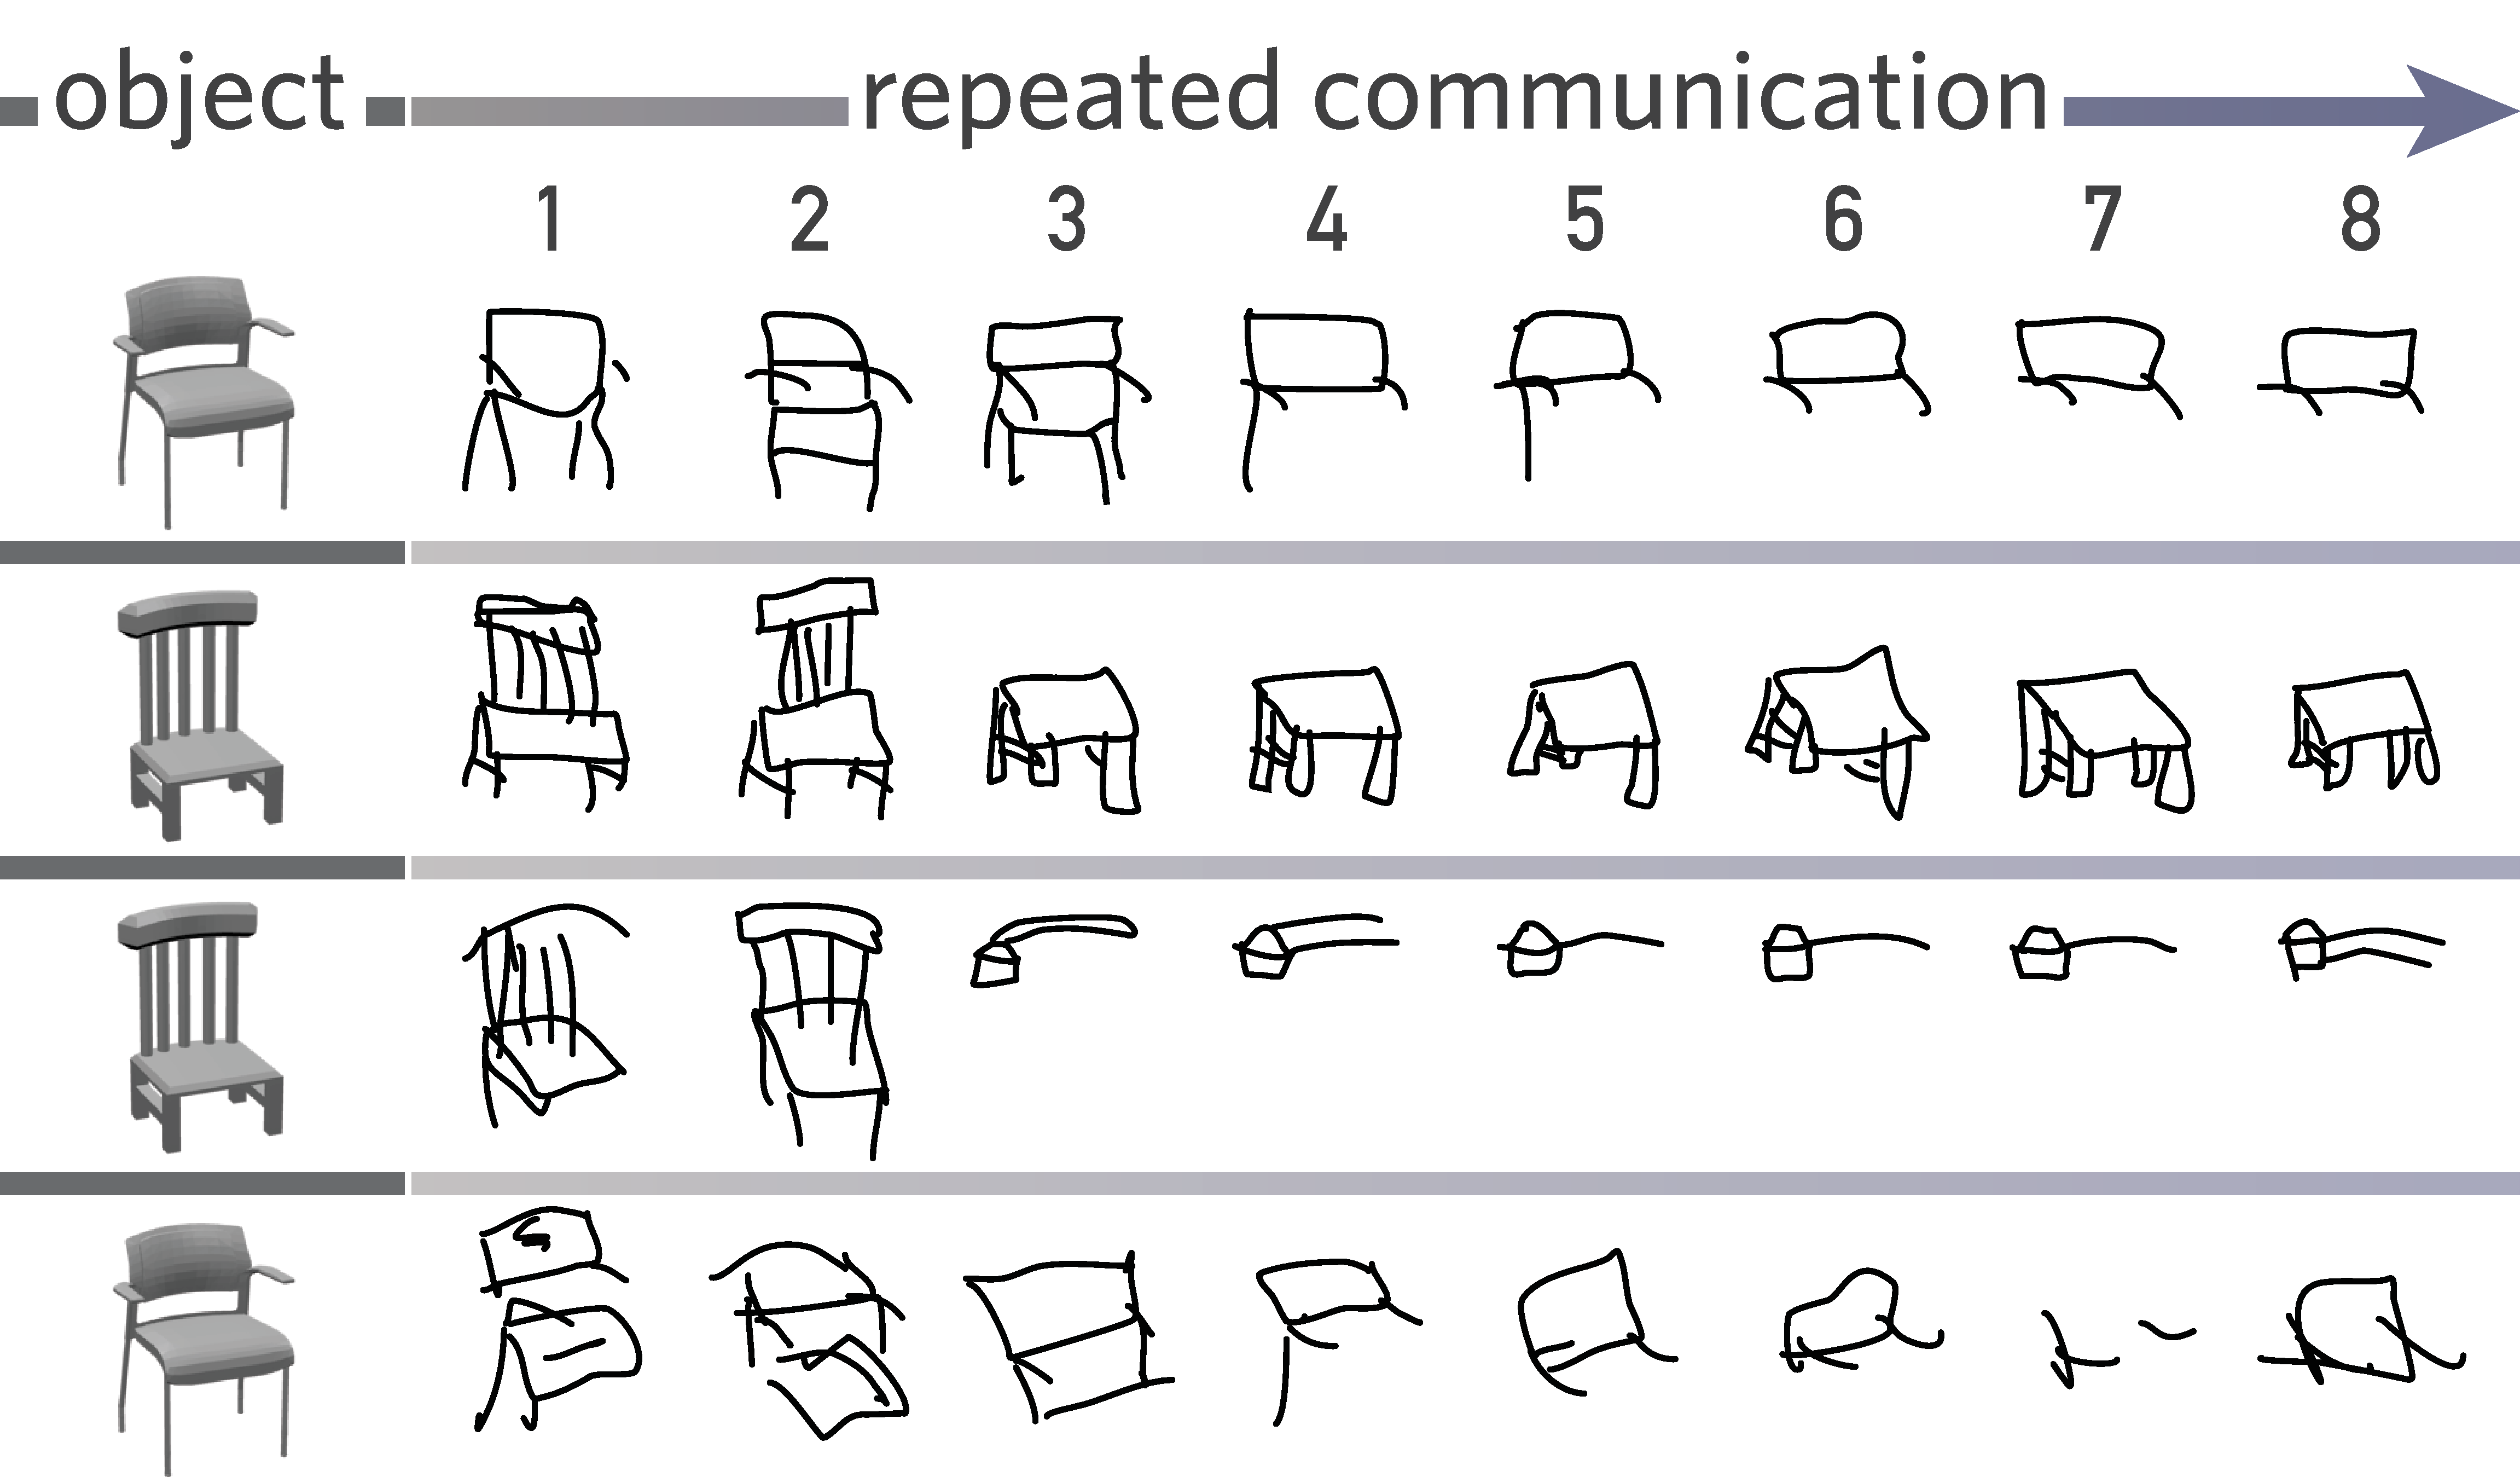
\includegraphics[width=0.99\linewidth]{figures/sketch_gallery.pdf}
\caption{Repeated visual communication about the same object.}
\label{sketch_gallery}
\end{figure}

How can these two perspectives be reconciled?
Our approach is to consider the joint contributions of visual information and social context in determining how drawings derive meaning \cite{abell2009canny}, and to propose that a critical factor affecting the balance between the two may be the amount of shared knowledge between communicators.
Specifically, we explore the hypothesis that accumulation of shared knowledge via extended visual communication may promote the development of increasingly schematic yet effective ways of depicting a physical object, even as these \textit{ad hoc} graphical conventions may be less readily apprehended by others who lack this shared knowledge.

To investigate this, we used an interactive drawing-based reference game in which two players repeatedly communicate about visual objects, and examined both how their task performance and the drawings they produced changed over time (see Fig. \ref{sketch_gallery}). 
Our approach was inspired by a large literature that has explored how extended interaction influences communicative behavior in several modalities, including language \cite{krauss1964changes,ClarkWilkesGibbs86_ReferringCollaborative,HawkinsFrankGoodman17_ConventionFormation}, gesture \cite{goldin1996silence,fay2014creating}, and drawings \cite{garrod_foundations_2007,fay2010interactive}.

% extra: Galantucci:2005uh,healey2007graphical,theisen2010systematicity

%% jefan: I want another sentence here, if possible, stating the limitations of this prior work that sets up the contributions of the current paper better.

There are three aspects of the current work that advances our prior understanding: \emph{first}, we include a control set of objects that were not repeatedly drawn, allowing us to measure the specific contribution of repeated reference; \emph{second}, we measure how strongly the visual properties of drawings drive recognition in the absence of interaction history, while equating other task variables; and \emph{third}, we employ recent advances in computational vision to quantitatively characterize changes in the high-level visual properties of drawings across repetitions.

%% Figure 1 around here: (A) Stimuli. (B) Task (Sketcher/Viewer interface)
\begin{figure*}
\begin{center}
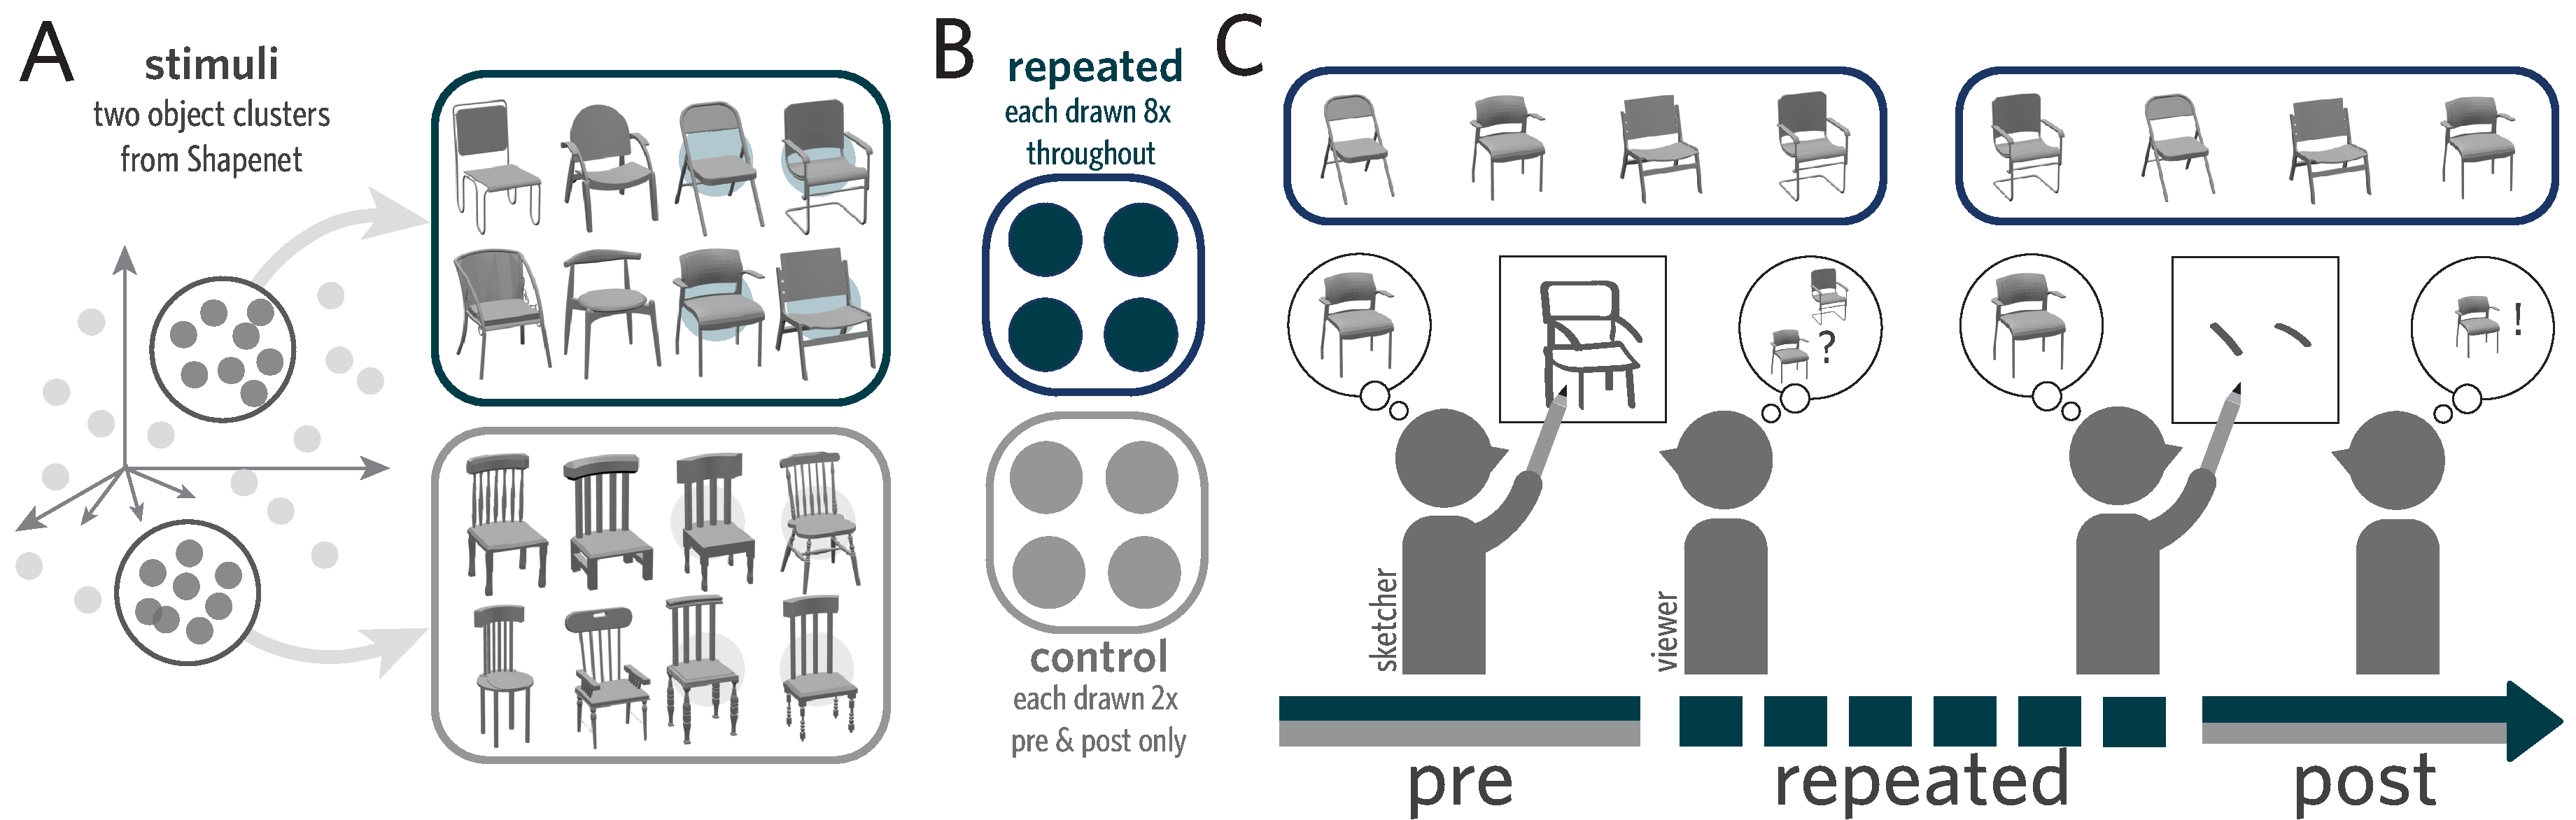
\includegraphics[width=0.95\linewidth]{figures/task_stimuli.pdf}
\caption{(A) Stimuli from ShapeNet (B) Each pair of participants was randomly assigned two sets of four objects, each set from one of these categories. (C) Repeated objects were drawn eight times throughout; control objects drawn once at the beginning and end of each interaction.}
\label{task_stimuli}
\vspace{-1em}
\end{center}
\end{figure*}

\section{Part I: How does repeated reference support successful visual communication?}

%% intro to this section
Our first goal was to understand how people learn to communicate about visual objects across repeated visual communication. 
To accomplish this, we developed a drawing-based reference game for two players. 
On each trial, both players were shown several images of objects, one of which was privately designated as the `target' to the sketcher. 
The sketcher's goal was to draw the target so that the viewer could select it from the context as quickly and accurately as possible. 
We hypothesized that learning would be \emph{object-specific}: that over repeated visual reference to a particular object, participants would discover ways of depicting that object more effectively relative to non-repeated control objects. 

% gains in communication efficiency for all objects, they were greater for the repeated objects, suggesting both task-level and object-level benefits of repeated communication.

% Our goal was to investigate how the accumulation of shared knowledge via extended visual communication between two people influences the drawings they produce and how well they communicate.
% Towards this end, we developed a visual communication task in which people repeatedly referred to familiar objects, but where pre-existing graphical conventions were unlikely to be sufficient to succeed.
% In line with prior studies of repeated verbal communication \cite<e.g>{ClarkWilkesGibbs86_ReferringCollaborative} and visual communication about verbal stimuli \shortcite<e.g.>{garrod_foundations_2007}, we hypothesized that repeated visual reference to a visual object would lead to more efficient communication about that object.
% Departing from prior studies, our experiment critically includes a control set of visual objects that are not repeatedly referenced, which allows us to measure the extent to which changes in efficiency are item-specific or attributable to task practice.


%% methods
\subsection{Methods: Visual communication experiment}

\subsubsection{Participants} We recruited 138 participants from Amazon Mechanical Turk and automatically matched them into 69 pairs.
%They were provided a base compensation of \$1.50 for participation and up to \$1.60 in bonus for high task performance.
Data from two pairs were excluded due to unusually low performance (i.e., accuracy $<$ 3 s.d. below the mean).
In this and subsequent experiments, participants provided informed consent in accordance with the Stanford IRB.\footnote{All materials and data will be made available upon un-blinding at \url{https://github.com/XXX}.}

\subsubsection{Stimuli}
%% provide justification for why we're using sets of similar objects
%% provide justification for why we're using images of real-world objects

In order to make our task sufficiently challenging, we sought to construct contexts of objects whose members were both geometrically complex and visually similar. 
To accomplish this, we sampled objects from the ShapeNet database \cite{chang2015shapenet}, which contains more than 51,300 3D mesh models of real-world objects. % belonging to 55 different object classes.
We restricted our search to 3096 objects belonging to the \texttt{chair} class, which is among the most diverse and abundant in ShapeNet. 
To identify groups of visually similar chairs, we first extracted high-level visual features from 2D renderings of these objects using a pre-trained deep convolutional neural network, VGG-19 \cite{simonyan2014very}.
Each of these 4096-dimensional feature vectors reflected VGG-19 activations to each object rendering in the second fully-connected layer (i.e., \texttt{fc6}).
We then applied dimensionality reduction (PCA) and $k$-means clustering on these feature vectors, yielding 70 clusters containing between 2 and 80 objects each.
Based on these clusters, we selected 2 categories of visually similar objects containing 8 exemplars each (Fig.~\ref{task_stimuli}A). 

\subsubsection{Task Procedure} 

%% Trial-level event structure
% Drawings were collected in the context of an online, sketching-based reference game using the framework described in \citeA{Hawkins15_RealTimeWebExperiments}.
% The game involved two players: a \textit{sketcher} who aims to help a \textit{viewer} pick out a target object from a set of distractor objects by representing it in a sketch.
On each trial, both participants were shown the same set of four objects in randomized locations.
One of the four objects was highlighted on the sketcher's screen to designate it as the target.
%% Trial-level objective of sketcher and viewer
Sketchers drew using their mouse cursor in black ink on a digital canvas (300 $\times$ 300 pixels; pen width = 5 pixels) embedded in their web browser. 
Each stroke was transmitted to the viewer's screen in real-time and sketchers were not able to delete previous strokes.
The viewer was allowed guess the identity of the drawn object by clicking one of the four objects as soon as they were confident, and participants received immediate feedback: the sketcher learned when and which object the viewer had clicked, and the viewer learned the true identity of the target. 
Finally, participants were incentivized to perform both quickly and accurately. 
Both participants earned an accuracy bonus for each correct response, and the sketcher was instructed to take no longer than 30 seconds to produce their drawings.
If the viewer responded under this time limit, participants also received a speed bonus inversely proportional to the time taken until the response.
%Otherwise, the viewer had no other means of communicating with the sketcher. 

%% Two conditions: repeated and control

% Each pair of participants was randomly assigned two of these categories, and only the 16 objects from these two categories appeared as drawing targets during their session.

\subsubsection{Design} 
For each pair, we randomly sampled two sets of four objects that served as contexts in the reference game: one was designated as a \emph{repeated} set while the other was a \emph{control} set (Fig.~\ref{task_stimuli}B)\footnote{In half of the pairs, the four control objects were from the same stimulus cluster as repeated objects; in the other half, they were from different clusters. We collapse across these groups in our analyses.}.% (N=34 for same; N=33 for different)
% These control objects were thus maximally perceptually similar to the repeated objects but were not repeatedly drawn and provided a tight baseline for object-specific effects. 
%In the other half of pairs (N=XX pairs), the repeated set contained four randomly sampled objects from one category and the control set contained four randomly sampled objects from the other category.
The experiment consisted of three phases (Fig.~\ref{task_stimuli}C).
During the central \textit{repeated reference} phase, there were six blocks of trials, and each of the four \emph{repeated} objects appeared as the target once in each block.
In a pre-test at the beginning of the experiment, and a post-test at the end, both repeated and control objects appeared once as targets (in their respective contexts) in randomly interleaved order. 
%Within this phase were six repetition cycles wherein each repeated object served as the target exactly once, and object order was randomized across repetition cycles. 
% These control objects still shared many perceptual features with the repeated objects, but provided a measure of the more generic effects of task practice.

\subsection{Results}

\begin{figure}
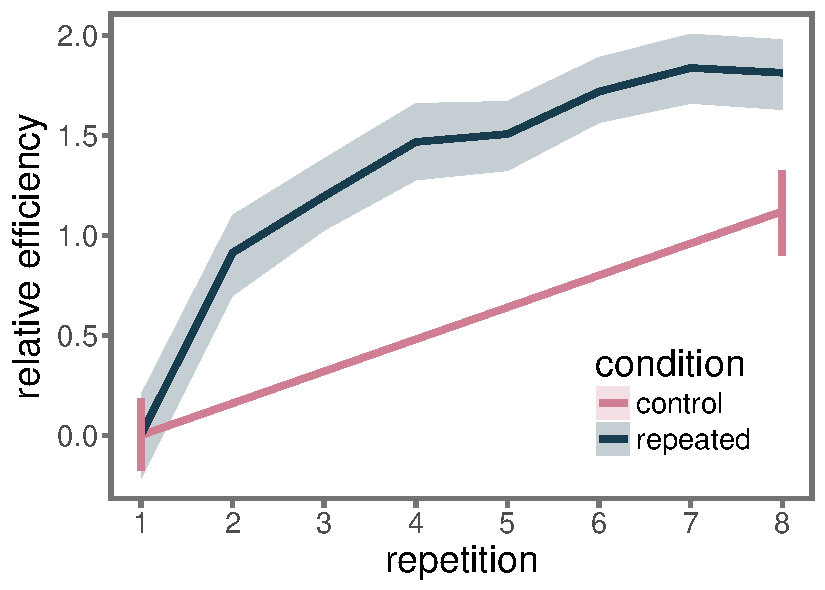
\includegraphics[width=\linewidth]{figures/refgame_BIS_timeseries.pdf}
\caption{Communication efficiency for repeated and control objects across repetitions. Efficiency combines both speed and accuracy, and is plotted relative to the first repetition.} 
% ... was computed using a metric that
\label{refgame_bis}
\end{figure}

Because objects were randomly assigned to repeated and control conditions, we expected no differences in task performance in the pre-test phase. 
We found that pairs identified the target at rates well above chance in this phase (75.7\% repeated, 76.1\% control, chance = 25\%), suggesting that they were engaged with the task but not at ceiling performance.
% n  empirical_stat      ci_lower            mean               ci_upper
%67	-0.003731343	-0.07089552	-0.001317164	0.07089552
However, we found no difference in accuracy across conditions (mean difference: 0.3\%, bootstrapped CI: $[-7\%, 7\%]$).

In order to measure how well pairs learned to communicate throughout the rest of their interaction, we used a measure of communicative efficiency \cite<the \emph{balanced integration score,}>{Liesefeld2018} that takes both accuracy (i.e., proportion of correct viewer responses) and response time (i.e., time taken to produce each drawing) into account.
This efficiency score is computed by first z-scoring the accuracy and response time variables to map these values to the same scale and then subtracting the standardized response time from standardized accuracy.
It is highest when pairs are both fast and accurate, and lowest when they make more errors and take longer, relative to their own performance on other trials.


% Formula: bis_score ~ phase * condition + (1 + phase * condition | gameID)
%    Data: input
% Fixed effects:
%                    Estimate Std. Error        df t value Pr(>|t|)
% (Intercept)        -0.42302    0.05473 125.82978  -7.730 2.97e-12 ***
% phase1             -1.44656    0.10112 137.22562 -14.306  < 2e-16 ***
% condition1          0.35670    0.14118  70.83601   2.527  0.01376 *
% phase1:condition1  -0.64821    0.20974  94.62722  -3.091  0.00262 **
% ---
% Signif. codes:  0 ‘***’ 0.001 ‘**’ 0.01 ‘*’ 0.05 ‘.’ 0.1 ‘ ’ 1

To evaluate changes in communicative efficiency, we fit a linear mixed-effects model with maximal random effect structure, including random intercepts, slopes, and interactions for each pair of participants.
We found that communicative efficiency increased for all targets between the \textit{pre} and \textit{post} phases ($b = 1.45,~t = 14.3,~p <0.001$), reflecting generalized improvements as a consequence of extended interaction.
Critically, however, this analysis also revealed a reliable interaction between phase and condition: communicative efficiency improved to a greater extent for repeated objects than control objects ($b = 0.648, ~t = 3.09,~p = 0.003$; see Figure \ref{refgame_bis}).
These results show that there are benefits of repeatedly communicating about an object that accrue specifically to that object, suggesting the formation of object-specific graphical conventions.

% the benefits of repeatedly communicating about an object accrue more strongly to that object
% show gains in communicative efficiency are to some extent specific to the objects that were repeatedly referenced

% Optional: We found a similar pattern of results when we used the number of strokes in each drawing instead of drawing time in our estimate of communicative efficiency.

% Thus, participants converged on simpler, faster, and more communicatively successful graphical conventions for repeated objects, which only partially transferred to other objects.

%We clearly see that while the cost of sketching decreases, the accuracy of the viewer's guess of which object the drawing is referring to increases, suggesting that this reduction is meaningful.

%% task-level and object-level benefits of extended communication.

%Successful communication was primarily quantified as the viewer's accuracy in identifying the target.
%The investment of time was measured as the length of time between the beginning of the first stroke to the completion of the final stroke in each sketch, and the investment of ink was measured in two ways: as the number of strokes used for each drawing and the proportion of the drawing canvas filled by ink.

%This ensures that the reduction in the drawing duration and number of strokes over time is not due to the players losing interest or becoming less motivated during the game.

\section{Part II: What explains gains in efficiency?}

The visual communication experiment established that pairs of participants coordinate on object-specific ways of depicting objects more efficiently across repetitions.
This raises the question: to what extent do these gains in communication efficiency reflect the accumulation of interaction-specific shared knowledge between a sketcher and viewer, as opposed to a combination of task practice and the inherent visual properties of the drawings?
To evaluate this question, we conducted two control experiments to measure the contribution of the latter.
In these experiments, naive participants performed a drawing recognition task in which they were presented with the final drawings from the communication experiment and guessed which of four objects it referred to.
Their task was thus the same as the viewer's in the communication experiment, except they knew their responses were not being provided as real-time feedback to the sketcher.

% , and they made their decision based on the final drawing, rather than being able to interrupt await additional information.

\subsection{Methods: Recognition Experiment}

\subsubsection{Participants}

245 participants recruited via AMT completed the experiment. Data from 22 participants were excluded who did not meet the criterion for accurate and consistent responding on attention-check trials.

\subsubsection{Task, Design, \& Procedure}
%How does efficiency of graphical communication, measured by how accurately and quickly the viewer can select the target intended by the sketcher, change when we change the degree of interaction specificity?
%Here, we define interaction specificity based on both temporal structure (path dependence) and partner specificity.
%Therefore, we design several experiments that measure the recognizability of drawings and reaction times produced in the drawing task by third-party observers.

On each trial, recognition participants were presented with a drawing paired with the same set of four objects that viewers had seen in the communication game, and guessed which object was the target.
Just as original viewers had been, they received an accuracy bonus for every correct response, and speed bonus inversely proportional to their response time.
To ensure task engagement, we included five identical attention-check trials that appeared once every eight trials.
Each attention-check trial presented the same set of objects and drawing, identified based on initial piloting to be the most consistently and accurately recognized by naive participants.
Participants who did not respond correctly on at least 4 out of 5 of these trials were excluded from subsequent analyses (N=22).

Each participant was randomly assigned to two groups: a \textit{yoked} group and a \textit{shuffled} group.
Those in the yoked group were matched with one pair in the communication experiment and viewed 40 drawings in the same sequence the original viewer had.
Participants in the shuffled group were matched with 10 distinct pairs from the communication experiment and viewed 4 drawings from each in turn, which appeared within the same repetition cycle as they had appeared originally.
At the trial level, both groups thus received exactly the same visual information and performed the task under the same incentives to respond quickly and accurately.
At the session level, both groups received exactly the same amount of practice recognizing drawings.
Thus any differences between the yoked and shuffled groups are attributable to whether drawings came from the same communicative interaction, which would support the accumulation of interaction-specific experience, or from several different interactions, where such accumulation would be minimal.

\subsection{Results}

\subsubsection{Accumulation of interaction-specific experience enhances recognition by third-party observers}

% Linear mixed model fit by REML. t-tests use Satterthwaite's method ['lmerModLmerTest']
% Formula: bis_relative ~ version * repetition + (1 + repetition | gameID)
%    Data: d.recog %>% filter(version %in% c("yoked", "shuffled"))

% Fixed effects:
%                             Estimate Std. Error        df t value Pr(>|t|)
% (Intercept)                  0.43214    0.06485 287.50472   6.663 1.36e-10 ***
% versionshuffled             -0.13284    0.08954 287.50472  -1.484    0.139
% repetition                   0.18430    0.01440 326.27439  12.801  < 2e-16 ***
% versionshuffled:repetition  -0.09715    0.01988 326.27439  -4.888 1.60e-06 ***
% ---
% Signif. codes:  0 ‘***’ 0.001 ‘**’ 0.01 ‘*’ 0.05 ‘.’ 0.1 ‘ ’ 1

We compared the yoked and shuffled groups by measuring changes in task performance on repeated objects using the same efficiency metric as we had previously.
We estimated the magnitude of these changes by fitting a linear mixed-effects model that included group (i.e., yoked vs. shuffled), repetition number (i.e., 1st through 8th), and their interaction, as well as random intercepts and slopes for each viewer/recognition participant.
This analysis revealed that recognition performance increased overall as a function of repetition number ($b = 0.184, ~t = 12.8, ~p < 0.001$), reflecting the general benefits of practice recognizing drawings and any inherent visual correspondences between between drawings and the target object.  %10^{-15}$
Critically, we also found a large and reliable interaction between group and repetition number: yoked participants improved to a substantially greater degree than shuffled participants ($b = 0.0972, ~t = 4.89, ~p<0.001$).
In addition, the yoked group was also more accurate overall at identifying the target object (yoked: 74.9\%, shuffled: 68.8\%, $~t = 3.59, ~p < 0.001$). %$0.0004
Taken together, these results suggest that third-party observers who could remain a `fly on the wall' throughout an entire interaction were able to take advantage of this continuity to quickly understand which object each drawing represented, relative to third-party observers who cycled through discontinuous excerpts from several different interactions in the same temporal order.

%% ACCURACY LMER
% Formula: accuracy ~ version + (1 | gameID)
% Fixed effects:
% Fixed effects:
%                  Estimate Std. Error        df t value Pr(>|t|)
% (Intercept)       0.74912    0.01228 221.00001  60.982  < 2e-16 ***
% versionshuffled  -0.06081    0.01696 221.00001  -3.586 0.000413 ***
% ---

%% ACCURACY MEANS
% communication	0.8745336
% yoked	0.7491156
% shuffled	0.6883013

% We found that communicative efficiency increased overall between the \textit{pre} and \textit{post} phases ($b = 1.45,~t = 14.3,~p <0.001$), reflecting generalized improvements as a consequence of extended interaction.
% Critically, this analysis also revealed a reliable interaction between phase and condition: communicative efficiency improved to a greater extent for repeated objects than control objects ($b = 0.648, ~t = 3.09,~p = 0.003$; see Figure \ref{refgame_bis}).

% We found a significant difference in recognizability: while there was some improvement across repetitions in the shuffled condition, likely attributable to a practice effect, they achieved significantly worse performance than participants in the yoked condition who saw the same drawings in their original context.

\subsubsection{Viewer feedback also contributes to gains in performance}

Because participants in the yoked group viewed drawings in exactly the same sequence as the original viewer had, we predicted that their recognition performance would improve to a comparable degree across repetitions.
However, unlike viewers in the communication game, these participants were unable to provide feedback to the sketcher, who could have used information about which object the viewer had selected and how quickly they were able to select it, in order to modify their drawings on subsequent repetitions \cite{schober_understanding_1989}.
Instead, yoked participants made their decision based only on the final drawing, and were unable to interrupt or await additional information from the sketcher if they were still uncertain.
As such, comparing the yoked and communication groups provides an estimate of the contribution of these viewer feedback channels to gains in performance.
We again measured changes in task performance on repeated objects using the same efficiency metric as we had previously, and estimated the magnitude of these changes by fitting a linear mixed-effects model that included group (i.e., communication vs. yoked), repetition (i.e., 1st through 8th), and their interaction as fixed effects, and maximal random effects structure, with random intercepts, slopes and interactions between group and repetition for each unique trial sequence.
This analysis revealed a strong overall effect of repetition ($b = 0.231, ~t = 12.8,~p < 0.001$; see Figure \ref{recog_bis}) and a weaker but reliable interaction with group membership ($b = -0.051, ~t = -2.178, ~p = 0.032$), showing that the yoked group improved nearly at the same rate as viewers in the communication experiment had, even in the absence of viewer feedback. %1x10^{-15}
However, viewers in the communication experiment were substantially more accurate overall at identifying the target object than yoked participants (communication: 87.5\%, yoked: 74.9\%, $t = 6.18, ~p < 0.001$), suggesting that these viewer feedback channels may help to boost performance in absolute terms. %1x10^{-8}$

%%% BIS LMER
% Linear mixed model fit by REML. t-tests use Satterthwaite's method ['lmerModLmerTest']
% Formula: bis_relative ~ version * repetition + (1 + version * repetition |      orig_gameID)
%    Data: d.recog %>% filter(version %in% c("communication", "yoked"))

% Fixed effects:
%                         Estimate Std. Error       df t value Pr(>|t|)
% (Intercept)              0.44820    0.07742 91.32869   5.790 9.87e-08 ***
% versionyoked            -0.03067    0.10700 78.98863  -0.287    0.775
% repetition               0.23067    0.01805 95.73466  12.777  < 2e-16 ***
% versionyoked:repetition -0.05088    0.02336 90.13517  -2.178    0.032 *
% ---
% Signif. codes:  0 ‘***’ 0.001 ‘**’ 0.01 ‘*’ 0.05 ‘.’ 0.1 ‘ ’ 1

%% ACCURACY MEANS
% communication	0.8745336
% yoked	0.7491156
% shuffled	0.6883013


%%% ACCURACY LMER
% Linear mixed model fit by REML. t-tests use Satterthwaite's method ['lmerModLmerTest']
% Formula: accuracy ~ version + (1 | gameID)
%    Data: d.acc

% Fixed effects:
%               Estimate Std. Error        df t value Pr(>|t|)
% (Intercept)    0.87453    0.01588 171.00000  55.086  < 2e-16 ***
% versionyoked  -0.12542    0.02028 171.00000  -6.184 4.46e-09 ***
% ---

\begin{figure}
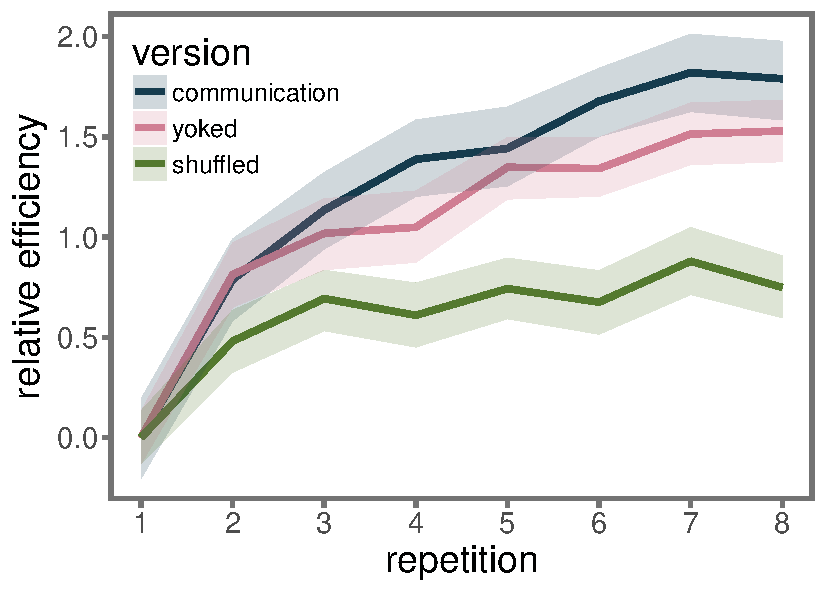
\includegraphics[width=\linewidth]{figures/recog_BIS_timeseries.pdf}
\caption{Recognition performance in control conditions; ribbons are 95\% CIs}
\label{recog_bis}
\end{figure}

\section{Part III: How do visual features of drawings change over the course of an interaction?}

\begin{figure*}
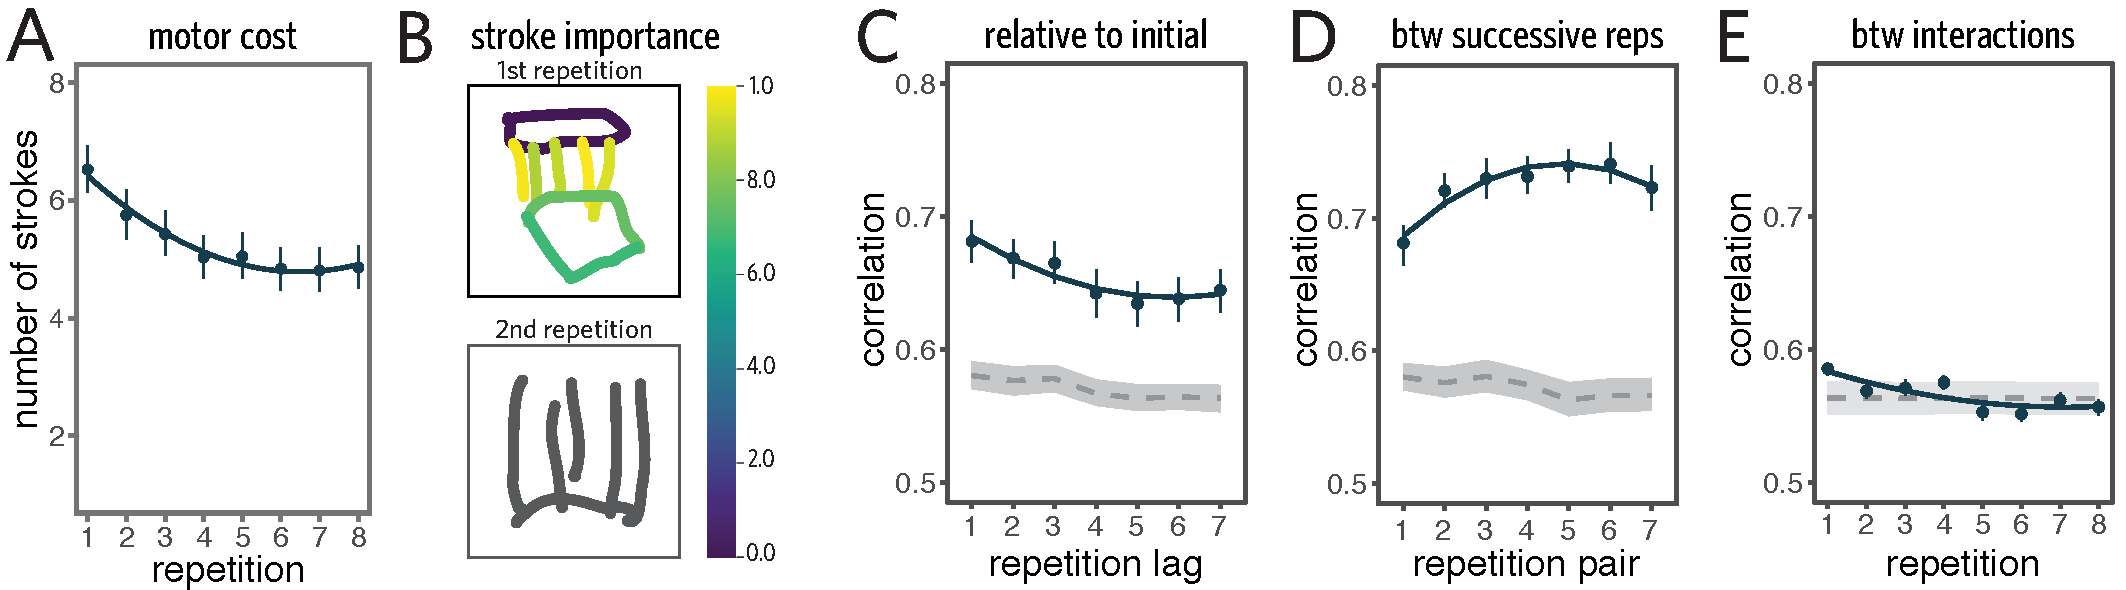
\includegraphics[width=0.96\linewidth]{figures/drawing_changes.pdf}
\caption{(A) Number of strokes in a drawing as function of repetition. (B) Visualizing importance of individual strokes in successive drawings. (C) Drawings change across repetitions, becoming increasingly dissimilar from initial drawing. (D) Drawings change more slowly later in interaction, becoming more internally consistent. (E) The same object is drawn increasingly dissimilarly in different interactions, suggesting multiple viable graphical conventions. Error ribbons represent 95\% CI, dotted lines represent permuted baseline.}
\label{within-across}
\end{figure*}

The results so far show that repeated visual communication establishes object-specific, interaction-specific ways of efficiently referring to objects.
An intriguing implication is that interacting pairs achieved this by gradually forming \textit{ad hoc} graphical conventions about what was relevant and sufficient to include in a drawing to support rapid identification of the target object. 
Here we explore this possibility by examining how the drawings themselves changed throughout an interaction.

Concretely, we investigated four aspects of how drawings may have changed that would reflect the increasing contribution of interaction-specific shared knowledge: \textit{first}, decreasing number of strokes used (i.e., reducing motor cost of each drawing); \textit{second}, increasing dissimilarity from the initial drawing produced (i.e., cumulative drift from the starting point); \textit{third}, increasing similarity between successive drawings (i.e., convergence on internally consistent ways of depicting objects); \textit{fourth}, increasing dissimilarity between drawings of the same object produced in different interactions (i.e., discovery of multiple viable solutions to coordination problem). 

% These control experiments establish that shared history with a particular sketcher is critical for the drawings to remain meaningful late in the game. 
% But what is happening over time to the visual features of the drawings themselves? 
% In this final section, we conduct finer-grained analyses of the dynamics of graphical representations across communication.

% First, replicating prior findings, we observed that the number of strokes used in each drawings decreased across repetitions, such that later drawings were systematically sparser than earlier ones (XXX; $p<.001$).

%% To analyze how the content of the sketches change over time, we extracted the high-level visual features of the drawings using a pre-trained convolutional neural network. 
%% Each sketch produced in our reference game data set was thus projected to a common 4,096-dimensional feature space given by the \texttt{fc6} layer of VGG. 

\subsection{Measuring visual similarity between drawings}

Measuring visual similarity between drawings relies upon having a principled approach to encoding their high-level visual properties.
Here we capitalize on recent work validating the use of deep convolutional neural network models, pre-trained on challenging visual tasks, to encode such perceptual content in drawings \cite{FanCommon2018}.
As we had when identifying clusters of similar object stimuli, we again used VGG-19 to extract 4096-dimensional feature vector representations for drawings of every object, in every repetition, from every interaction. 
Using this feature basis, we compute the similarity between any two drawings as the Pearson correlation between their feature vectors (i.e., $r_{ij} =  \nicefrac{cov(\vec{r}_{i}, \vec{r}_{j})}{\sqrt{var(\vec{r}_{i}) \cdot var(\vec{r}_{j})}}$).

\subsection{Results}
\subsubsection{Fewer strokes across repetitions} 

A straightforward explanation for the gains in communication efficiency observed in Part I is that sketchers were able to use fewer strokes per drawing to achieve the same level of recognition accuracy by the viewer.
In support of this account, a linear mixed-effects model with random slopes and intercepts for each sketcher showed that the number of strokes in drawings of repeated objects decreased steadily as a function of repetition ($b = -0.216, ~t = -6.00, ~p < .001$; Fig. \ref{within-across}A), suggesting that pairs were increasingly able to rely upon shared knowledge to communicate efficiently. 
This result raises question about which strokes are preserved across successive repetitions during the formation of graphical conventions. 
In ongoing work, we are investigating the ``importance'' of each stroke within a drawing for explaining similarity to the next repetition's drawing of that object, by re-rendering the drawing without each stroke and computing its feature-based similarity to the next drawing (Fig. \ref{within-across}B). 

% Linear mixed model fit by REML. t-tests use Satterthwaite's method ['lmerModLmerTest']
% Formula: numStrokes ~ repetition + (1 + repetition | gameID)
%    Data: d %>% filter(condition == "repeated")

% Fixed effects:
%             Estimate Std. Error       df t value Pr(>|t|)    
% (Intercept)  6.04384    0.30301 66.00001  19.946  < 2e-16 ***
% repetition  -0.21562    0.03595 66.00001  -5.998 9.32e-08 ***


% \jefan{Original version of this paragraph is nice but needs to be heavily streamlined.}
% As a qualitative first step toward answering this question, we conducted a stroke lesion analysis to visualize the ``importance'' of each stroke in determining its similarity to the next repetition's sketch.
% Specifically, we operationalized importance by re-rendering the drawing without each stroke and computing the feature-based similarity to the next drawing (see Fig. \ref{within-across}D).
% We observed that in the earlier drawing, strokes that seemed to refer to similar object parts as the remaining strokes in the later drawing were most important: lesioning them was the biggest blow to the drawing similarity.  

%The color of a stroke in a drawing corresponds to the similarity of the drawing to its successor when removing that stroke from the sketch.

\subsubsection{Increasing dissimilarity from initial drawing}

Mirroring the observed reduction in the number of strokes across repetitions, we hypothesized that there was also cumulative change in the perceptual content of drawings across repetitions. 
Concretely, we predicted that drawings would become increasingly dissimilar from the initial depiction. 
We tested this prediction in a mixed-effect regression model including linear and quadratic terms for repetition as well as intercepts for each target and pair.
We found a significant decrease in similarity to the initial round across successive repetitions, $b = -0.62,~t = -5.59, ~p < 0.001$; Fig.~\ref{within-across}C, suggesting that later drawings had moved to a different region of visual feature space. 
However, since the entire distribution of drawings may have drifted to a different region of the visual feature space for generic reasons (i.e., because they were sparser overall), we conducted a stricter permutation test.  
We scrambled drawings across \emph{interactions} but within each repetition and target.
The true effect $(t = -5.59$) fell outside this null distribution $(95\%~CI= [-3.53 -0.88], ~p < .001)$, showing that successive drawings by the same sketcher deviated from their own initial drawing to a greater degree than would be expected due to generic differences between drawings made in different repetitions. 

\subsubsection{Increasing internal consistency within interaction}

At the same time as we noticed drawings growing steadily different from the initial sketch, this displacement also seemed to \emph{slow down} considerably.
In other words, while there may be major revisions or simplifications of drawings in early rounds, sketchers may eventually settle into  increasingly \emph{internally consistent} or stable conventions.
We examined this prediction by computing the pairwise similarity of drawings drawn on \emph{successive rounds} of the same target object by the same sketcher.
We found that the similarity of successive drawings \emph{increases} strongly over time ($b = 0.53,~t = 5.03$; see Figure \ref{within-across}) in a mixed effects regression with random intercepts for both sketcher and target.
Again, as a baseline, we considered the null distribution of slope $t$ values produced by first scrambling drawings across pairs in order to disrupt the consistency within games.
The true effect was significantly greater than this null distribution, $p < .001$, which actually tended in the opposite direction $CI = [-3.21, -0.60]$.

\subsubsection{Different sketchers draw the same object in increasingly different ways}

The shuffled condition of our control experiments suggested that conventions were \emph{interaction-specific}; we made the further prediction that while early drawings may be more strongly constrained by a shared target image, later drawings may be more \emph{variable} as pairs settle into multiple equilibria.
In other words, the \emph{visual features} of drawings from different pairs for the same target may diverge from one another over the course of the game.
We tested this prediction by computing the mean pairwise similarity of drawings of each target \emph{across games} on each repetition.
In a mixed-effects regression including linear and quadratic terms, we found a weak effect of repetition on pairwise drawing similarity ($b = -1.4, ~t = -2.5$; see Fig. \ref{within-across})  after including random slopes and intercepts for targets and game pairs. %and quadratic ($b= 0.42, t = 3.9$)
We conducted a permutation test to non-parametrically compare this observed decrease in similarity with what would be expected from disrupting the temporal structure of our data.
For each pair and target object, we scrambled drawing identifiers across repetitions 1000 times to generate a null distribution of $t$ values $(CI = [-0.57, 0.60])$, under which the observed decrease was highly unlikely,~$p~<~0.001$.

% should we still include the lesion-early lesion-late?

\subsection{Discussion}

% Summary paragraph
In this paper, we investigated the joint contributions of visual information and social context in determining the meaning of drawings.
We observed in an interactive Pictionary-style communication game that pairs discover increasingly sparse yet effective graphical representations as they repeatedly depict the same objects.
Through a series of control experiments, we demonstrated that these simpler drawings were harder for independent viewers to recognize without sharing the history of interaction with the same sketcher.

Furthermore, by analyzing the high-level visual features of drawings, we found that they became increasingly consistent within an interaction, but that different pairs discovered different equilibria in the space of viable graphical conventions. 
Taken together, our findings suggest that repeated visual communication promotes the emergence of depictions whose meanings are increasingly determined by shared knowledge rather than their visual properties alone.

% highlighting generative innovations relative to previous work
% (i.e. we're not just doing reproducing the same thing but with better controls & analyses; we're exploring a different part of the space)
While our results build on previous work in graphical convention formation \cite{garrod_foundations_2007,fay2010interactive}, there were two key differences in our paradigm.
First, we used \emph{images} as the targets of reference instead of more verbal concepts like ``art gallery'' or ``Robert de Niro.''
We expected this choice to initially ground different pairs more strongly in the same visual features and reduce variance across pairs; that we still observed modestly diverging representations across pairs is an even stronger testament to the role of social context in drawing production.
Furthermore, because both drawings and target objects share the same modality, future work should directly examine the similarity of drawings to the target images to measure the effect of iconicity.
Second, our \emph{feedback mechanism} differed from those that were the focus of prior work.
Viewers saw the drawing being produced in real-time and interrupted sketching as soon as they made their selection, then both players saw the selection and correct target.
This interruption mechanism provides \emph{more} information than synchronously making a selection after the sketcher decided to stop drawing, but \emph{less} information than allowing viewers to jointly drawing on the same canvas; future work should directly compare these intermediate gradations of feedback.

Our work also leaves open several hypotheses about \emph{how} people are deciding which strokes to preserve or drop on each trial.
According to one account, sketchers may be guided a \emph{primacy} bias where they drop out later, detail-providing strokes to preserve their initial strokes.
A second possibility is that they are guided by a \emph{recency} bias: when a particular drawing is successful, they keep the final strokes they put down and drop out earlier ones.
Finally, the temporal structure of drawings may not matter and they could simply be dropping random strokes, or the least informative strokes.
An important task for future work is to distinguish between these possibilities using lesion analyses like those above, or more fine-grained computational models of drawing generation.
\rdh{Need a final sentence, maybe along the lines of: ``understanding the fine-grained factors that drive graphical convention formation is foundational for understanding how non-photorealistic abstractions derive their meaning.''}

%\vspace{-.30cm}
%\section{\bf Acknowledgments}
%\small
%RXDH was supported by the Stanford Graduate Fellowship and the National Science Foundation Graduate Research Fellowship (DGE-114747). NDG was supported by ONR grant N000141310341 and a Sloan Foundation fellowship.
%\vspace{-.20cm}
\bibliographystyle{apacite}

\setlength{\bibleftmargin}{.125in}
\setlength{\bibindent}{-\bibleftmargin}

\bibliography{references}


\end{document}
